%!TEX root = ../../main.tex

\section{Experiments} \label{4_results}

We evaluate the Mutex Watershed on the challenging task of 
neuron segmentation in electron microscopy (EM) image volumes.
This application is of key interest in connectomics, a field of 
neuro-science that strives to reconstruct neural wiring digrams spanning complete central nervous systems. The task requires segmentation of neurons from electron microscopy images of neural tissue -- a challenging endeavor, since segmentation has to be based only on boundary information (cell membranes) and some of the boundaries are not very pronounced. Besides, cells contain membrane-bound organelles, which have to be suppressed in the segmentation. Some of the neuron protrusions are very thin, but all of those need to be preserved in the segmentation to arrive at the correct connectivity graph. While a lot of progress is being made, currently only manual tracing or proof-reading yields sufficient accuracy for correct circuit reconstruction \cite{schlegel2017Learning}.

We validate the Mutex Watershed algorithm on the most popular neural segmentation challenge: ISBI2012 \cite{isbi2012challenge}. We estimate the edge weights using a CNN as described in Section \ref{4_cnn} and compare with other entries in the leaderboard as well as with other popular post-processing methods for the same network predictions in Section \ref{4_isbi}. 

%The connectomics community has set up three popular segmentation challenges: ISBI2012 \cite{Isbi}, SNEMI3D \cite{snemi} and CREMI \cite{cremi}. The SNEMI3D challenge has been solved by \cite{lee2016superhuman} and the groundtruth for the test dataset has been published in \cite{Kasthuri2015}. We validate the Mutex watershed algorithm on the remaining two challenges. For the ISBI challenge, we estimate the edge weights using a CNN as described in 4.2 and compare against several other post-processing methods applied to the same network predictions (4.3). For the CREMI challenge, we re-purpose the predictions of the CNN used for the current leading entry (UnetLMC2) and directly compare to the lifted multicut post-processing used there (4.4). 

\subsection{Estimating edge weights with a CNN} \label{4_cnn}
The common first step to EM segmentation is to predict which pixels belong to a cell membrane using a CNN. Different post-processing methods are then used to obtain a segmentation, see \autoref{2_rel_work} for an overview of such methods.
%from simple thresholding to globally optimal lifted multicut. The prediction can be done globally \cite{everyone} or on the cell by cell basis \cite{Januszewski2017}.
The CNN can either be trained to predict boundary pixels \cite{ciresan_12_deep-em-segmentation,beier2017multicut} or undirected affinities \cite{lee2017superhuman,funke2018large} which express how likely it is for a pixel to belong to a different cell than its neighbors in the 6-neighborhood. In this case, the output of the network contains three channels, corresponding to left, down and next imaging plane neighbors in 3D. The affinities do not  have to be limited to immediate neighbors -- in fact, \cite{lee2017superhuman} have shown that introduction of long-range affinities is beneficial for the final segmentation even if they are only used to train the network. Building on the work of \cite{lee2017superhuman}, we train a CNN to predict short- and long-range affinities and then use those directly as weights for the Mutex Watershed algorithm. 

We estimate the affinities / edge weights for the neighborhood structure shown in Figure \ref{fig:connectivity}. To that end, we define local attractive and long-range repulsive edges. When attractive edges are only short-range, the solution will consist of spatially connected segments that cannot comprise ``air bridges''. This holds true for both (lifted)~multicut and for Mutex Watershed. We use a different pattern for in-plane and between-plane edges due to the great anisotropy of the data set. In more detail, we pick a sparse ring of in-plane repulsive edges and additional longer-range in-plane edges which are necessary to split regions reliably (see Figure \ref{fig:2d-connection}).
We also added connections to the indirect neighbors in the lower adjacent slice to ensure correct 3D connectivity (see Figure \ref{fig:3d-connection}). In our experiments, we pick a subset of repulsive edges, by using strides of 2 in the XY-plane in order to avoid artifacts caused by occasional very thick membranes. Note that the stride is not applied to local (attractive) edges, but only to long-range (repulsive) edges. The particular pattern used was selected after inspecting the size of typical regions. The specific pattern is the only one we have tried and was {\it not} optimized over.
%This reduces artifacts in form of single pixel segments due to thick boundaries.
%It also decrease the runtime of the Mutex Watershed by reducing the total number of edges considered by Algorithm \ref{algo_code}.

In total, $C^+$ attractive and $C^-$ repulsive edges are defined for each pixel, resulting in $C^+ + C^-$ output channels in the network. 
We partition the set of attractive / repulsive edges into subsets $H^+$ and $H^-$ that contain all edges at a specific offset:
$\label{edgesets}
    E^+ = {\bigcup_{c=1}^{C^+}} H^+_{c}$ for attractive edges, with $H^{-}$ defined analogously. 
Each element of the subsets $H^+_{c}$ and $H^-_{c}$ corresponds to a specific channel predicted by the network. We further assume that weights take values in $[0,1]$.% and adopt the same conventions for attractiveness / repulsion as in section \ref{3_methods}. 

\subsubsection*{Network architecture and training}
We use the 3D U-Net \cite{ronneberger_15_u-net, cciccek20163d} architecture, as proposed in \cite{funke2018large}. %It is illustrated in Figure \ref{fig:architecture}.

Our training targets for attractive / repulsive edges $\gt{w}^\pm$ can be derived from a groundtruth label image $\gt{L}$ according to
\begin{equation}
    \gt{w}^+_{e=(i, j)} = \begin{cases}
        1 , &\text{ if } \gt{L}_i = \gt{L}_j\\
        0 , & \text{otherwise}
    \end{cases}\quad
\end{equation}
\begin{equation}
    \gt{w}^-_{e=(i, j)} = \begin{cases}
        0 , &\text{ if } \gt{L}_i = \gt{L}_j\\
        1 , & \text{otherwise}
    \end{cases}
\end{equation}

Here, $i$ and $j$ are the indices of vertices / image pixels.
Next, we define the loss terms

\begin{equation} \label{dice_plus}
    \mathcal{J}^+_{c} = - \frac{\sum_{e \in H^+_{c}} (1 - w^+_e) (1 - \gt{w}^+_e)}{\sum_{e \in H^+_{c}} ((1 - w^+_e)^2 + (1 -\gt{w}^+_e)^2)} 
\end{equation}\label{dice_minus}
\begin{equation}
 \mathcal{J}^-_{c} = - \frac{\sum_{e \in H^-_{c}} w^-_e {\gt{w}^-_e}}{\sum_{e \in H^-_{c}} ((w^-_e)^2 + (\gt{w}^-_e)^2)}
\end{equation}
for attractive edges (i.e. channels) and repulsive edges (i.e. channels).

\begin{figure}
    \centering
    \begin{subfigure}[b]{0.95 \linewidth}
    \centering
    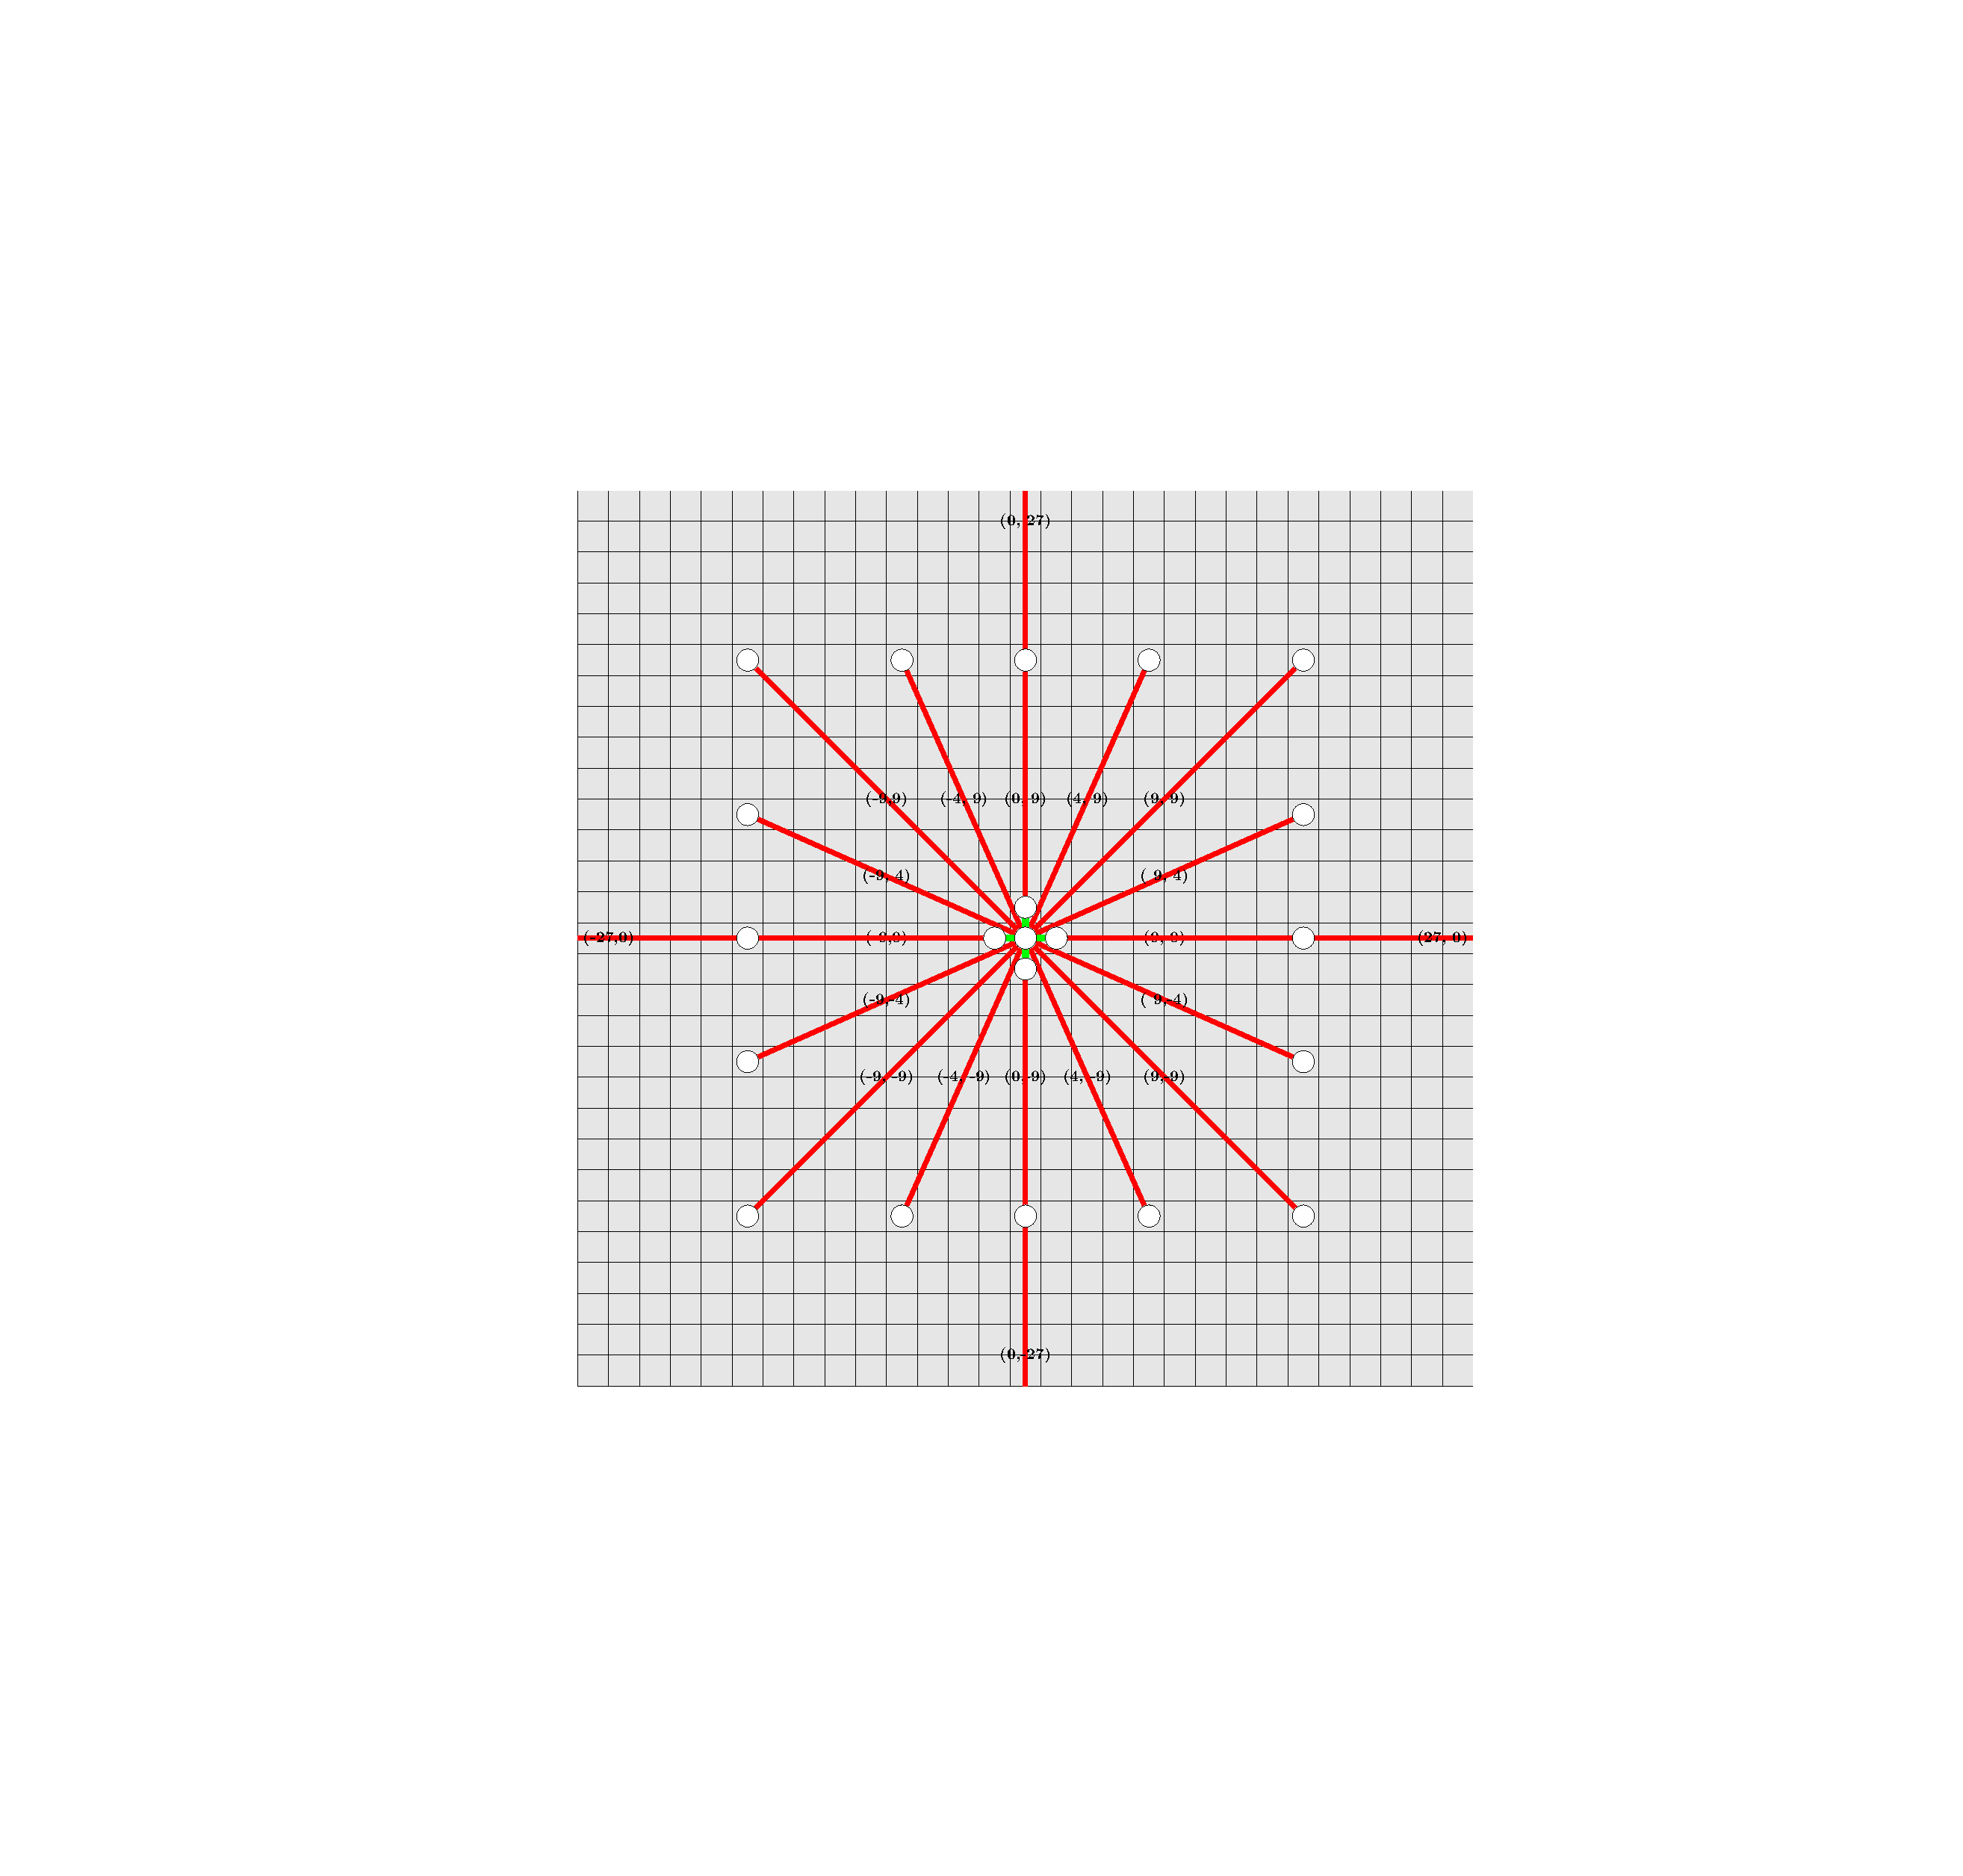
\includegraphics[width=0.9\linewidth]{figures/MWS/images/2d_connection.pdf}%
    \caption{XY-plane neighborhood with local attractive edges (green) and
     sparse repulsive edges (red) with approximate radius 9 and further long-range connections with distance 27}\label{fig:2d-connection}
    \end{subfigure}
    \par\bigskip
    \begin{subfigure}[b]{0.95 \linewidth}
    \centering
    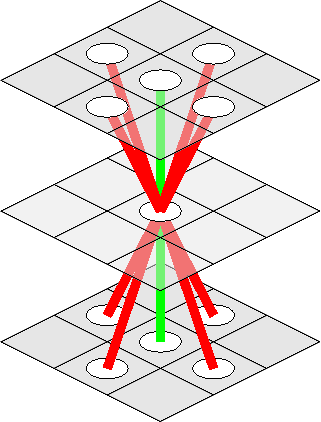
\includegraphics[width=0.4\linewidth]{figures/MWS/images/3d_connection3.pdf}
    \caption{Due to the great anisotropy of the data we limit the Z-plane edges to a distance of 1. The direct neighbors are attractive, whereas the indirect neighbors are repulsive.}\label{fig:3d-connection}
    \end{subfigure}%
    \caption{Local neighborhood structure of attractive~(green) and repulsive~(red) edges in the Mutex Watershed graph.}
    \label{fig:connectivity}
\end{figure}
Equation \ref{dice_plus} is the S{\o}rensen-Dice coefficient \cite{dice1945measures,sorensen1948method} formulated for fuzzy set membership values.
During training we minimize the sum of attractive and repulsive loss terms $\mathcal{J} = \sum_{c}^{C^+} \mathcal{J}^{+}_{c} + \sum_{c}^{C^-} \mathcal{J}^{-}_{c}$. This corresponds to summing up the channel-wise S{\o}rensen-Dice loss. 
The terms of this loss are robust against prediction and / or target sparsity, a desirable quality for neuron segmentation: since membranes are locally two-dimensional and thin, they occupy very few pixels in three-dimensional the volume. 
More precisely, if $w^{+}_e$ or $\gt{w}^{+}_e$ (or both) are sparse, we can expect the denominator $\sum_e(({w^{+}_e})^2 + (\gt{w}^+_e)^2)$ to be small,
which has the effect that the numerator is adaptively weighted higher. 
In this sense, the S{\o}rensen-Dice loss at every pixel $i$ is conditioned on the global image statistics, which is not the case for a Hamming-distance based loss like Binary Cross-Entropy or Mean Squared Error. 

We optimize this loss using the Adam optimizer \cite{kingma2014adam} and additionally condition learning rate decay on 
the Adapted Rand Score \cite{isbi2012challenge} computed on the training set every 100 iterations.
During training, we augment the data set by performing in-plane rotations by multiples of 90 degrees, flips along the X- and Y-axis as well as elastic deformations.
At prediction time, we use test time data augmentation, presenting the network with
seven different versions of the input obtained by a combination of rotations by a multiple of 90 degrees, axis-aligned flips and transpositions.
The network predictions are then inverse-transformed to correspond to the original image, and the results averaged.

\subsection{ISBI Challenge} \label{4_isbi}

The ISBI 2012 EM Segmentation Challenge \cite{isbi2012challenge} is the neuron segmentation challenge 
with the largest number of competing entries.
The challenge data contains two volumes of dimensions 1.5 $\times$ 2 $\times$ 2 microns and 
has a resolution of 50 $\times$ 4 $\times$ 4 nm per pixel. The groundtruth is provided as binary membrane
labels, which can easily be converted to a 2D, but not 3D segmentation. To train a 3D model, we follow the procedure
described in \cite{beier2017multicut}. 
\captionsetup[subfigure]{justification=centering, singlelinecheck=off}
\begin{figure}
\centering
    \begin{subfigure}[t]{0.46 \linewidth}
        \centering
        \includegraphics[width=0.98\textwidth]{figures/MWS/images/damws_2.png}
        \caption{Mutex Watershed} \label{fig:mws1}
    \end{subfigure}\hspace{0.5cm}
    \vspace{0.3cm}
    \begin{subfigure}[t]{0.46 \linewidth}
        \centering
        \includegraphics[width=0.98\textwidth]{figures/MWS/images/damws_1.png}
        \caption{Mutex Watershed} \label{fig:mws2}
    \end{subfigure}
    \vspace{0.3cm}
    \begin{subfigure}[t]{0.46 \linewidth}
        \centering
        \includegraphics[width=0.98\textwidth]{figures/MWS/images/mclr_2.png}
        \caption{Multicut partitioning based segmentation~(MC-FULL)} \label{fig:mc_full}
    \end{subfigure}\hspace{0.5cm}
    \begin{subfigure}[t]{0.46 \linewidth}
        \centering
        \includegraphics[width=0.98\textwidth]{figures/MWS/images/thresholded_1.png}
        \caption{Thresholding of local boundary maps ~(THRESH)} \label{fig:thresh}
    \end{subfigure}%
    
    \begin{subfigure}[t]{0.46 \linewidth}
        \centering
        \includegraphics[width=0.98\textwidth]{figures/MWS/images/ws_2.png}
        \caption{Watershed, seeded at local minima of the smoothed input map~(WS)} \label{fig:ws}
    \end{subfigure}\hspace{0.5cm}%
    \begin{subfigure}[t]{0.46 \linewidth}
        \centering
        \includegraphics[width=0.98\textwidth]{figures/MWS/images/wsdt_22.png}
        \caption{Distance Transform Watershed~(WSDT)} \label{fig:wsdt}
    \end{subfigure}
    % \vspace{-0.4cm}
    \caption{Mutex Watershed and baseline segmentation algorithms applied on the ISBI Challenge test data. Red arrows point out major errors. Orange arrows point to difficult, but correctly segmented regions. All methods share the same input maps.}
    \label{fig:isbi-examples}
\end{figure}% \captionsetup[figure]{justification=centering, singlelinecheck=off}
% \begin{figure}
% \centering
%     \begin{subfigure}[t]{0.45 \linewidth}
%         \centering
%         \includegraphics[width=0.91\textwidth]{images/damws_2.png}
%         \caption{Mutex Watershed} \label{fig:mws1}
%     \end{subfigure}\hspace{0.5cm}
%     \begin{subfigure}[t]{0.45 \linewidth}
%         \centering
%         \includegraphics[width=0.91\textwidth]{images/damws_1.png}
%         \caption{Mutex Watershed} \label{fig:mws2}
%     \end{subfigure}

%     \begin{subfigure}[t]{0.45 \linewidth}
%         \centering
%         \includegraphics[width=0.91\textwidth]{images/mclr_2.png}
%         \caption{Multicut partitioning based segmentation~(MC-FULL)} \label{fig:mc_full}
%     \end{subfigure}\hspace{0.5cm}
%     \begin{subfigure}[t]{0.45 \linewidth}
%         \centering
%         \includegraphics[width=0.91\textwidth]{images/thresholded_1.png}
%         \caption{Thresholding of local boundary maps ~(THRESH)} \label{fig:thresh}
%     \end{subfigure}%
    
%     \begin{subfigure}[t]{0.45 \linewidth}
%         \centering
%         \includegraphics[width=0.91\textwidth]{images/ws_2.png}
%         \caption{Watershed, seeded at local minima of the smoothed input map~(WS)} \label{fig:ws}
%     \end{subfigure}\hspace{0.5cm}%
%     \begin{subfigure}[t]{0.45 \linewidth}
%         \centering
%         \includegraphics[width=0.91\textwidth]{images/wsdt_22.png}
%         \caption{Distance Transformed Watershed~(WSDT)} \label{fig:wsdt}
%     \end{subfigure}
%     % \vspace{-0.4cm}
%     \caption{Mutex Watershed and baseline segmentation algorithms applied on the ISBI Challenge test data. Red arrows point out mayor errors. Orange arrows point to difficult, but correctly segmented regions. All methods share the same input maps.}
%     \label{fig:isbi-examples}
% \end{figure}

The test volume has private groundtruth; results can be submitted to the leaderboard.
They are evaluated based on the Adapted Rand Score (Rand-Score) and the Variation of Information Score (VI-Score) \cite{isbi2012challenge}.%, separately for each 2D plane. 
%The results are evaluated separately for the individual 2D imaging planes with final score corresponding to the average over the planes.

Our method holds the top entry in the challenge's leader board\footnote{{\href{url}{http://brainiac2.mit.edu/isbi\_challenge/leaders-board-new}}} at the time of submission, see Table \ref{tab:isbi-leaderboard}.
This is especially remarkable insofar as it is simpler than the methods holding the other 
top entries. \RED{Three out of four rely on a CNN to predict boundary locations and postprocess
its output with the complex pipeline described in \cite{beier2017multicut}.} 
This post-processing first generates superpixels via distance transform watersheds.
Then it computes a merge cost for local and long-range connections between superpixels.
Based on this, it defines a lifted multicut partioning problem that is solved approximately.
In contrast, our method finds an optimal solution of its objective purely on the pixel level.

\subsubsection*{Comparison with other segmentation methods}
The weights predicted by the CNN described above can be post-processed directly by the Mutex Watershed algorithm. To ensure a fair comparison, we transform the same CNN predictions into a segmentation using basic and state-of-the-art post-processing methods. 
We start from simple thresholding (THRESH) and seeded watershed. Since these cannot take long-range repulsions into account, we generate a boundary map by taking the maximum\footnote{The maximum is chosen to preserve boundaries.} values over the attractive edge channels. Based on this boundary map, we introduce seeds at the local minima (WS) and at the maxima of the smoothed distance transform (WSDT). For both variants, the degree of smoothing was optimized such that each region receives as few seeds as possible, without however causing severe under-segmentation. The performance of these three baseline methods in comparison to Mutex Watershed is summarized in Table~\ref{tab:isbi-baselines}. The methods were applied only in 2D, because the
high degree of anisotropy leads to inferior results when applied in 3D.
In contrast, the Mutex Watershed can be applied in 3D out of the box and yields significantly better
2D segmentation scores.

Qualitatively, we show patches of results in Figure \ref{fig:isbi-examples}.
The major failure case for WS (Figure \ref{fig:ws}) and WSDT (Figure \ref{fig:wsdt})
is over-segmentation caused by over-seeding a region.
The major failure case for THRESH is under-segmentation due to week boundary evidence (see Figure \ref{fig:thresh}).
In contrast, the Mutex Watershed produces a better segmentation, only causing minor over-segmentation (see Figure \ref{fig:mws1}, Figure \ref{fig:mws2}).

Note that, in contrast to most pixel-based postprocessing methods, our algorithm can take long
range predictions into account. To compare with methods which share this property, we turn to the multicut and lifted multicut-based partitioning for neuron segmentations as
introduced in \cite{andres_12_globally} and \cite{horvnakova2017analysis}. As proposed in \cite{andres2012globally}, we compute costs corresponding to edge cuts from the affinities estimated by the CNN via:
\begin{equation}
\label{mc_costs}
    s_e = \begin{cases}
        \log \frac{w^+_e}{1 - w^+_e} , &\text{ if } e \in E^+ \\
        \log \frac{1 - w^-_e}{w^-_e}, & \text{otherwise},
    \end{cases}
\end{equation}
We set up two multicut problems: the first is induced only by the short-range edges (MC-LOCAL), the other by short- and long-range edges together (MC-FULL). Note that the solution to the full connectivity problem can contain ``air bridges'', i.e. 
pixels that are connected only by long-range edges, without a path along the local edges connecting them.
However, we found this not to be a problem in practice.
In addition, we set up a lifted multicut (LMC) problem from the same edge costs.

Both problems are NP-hard, hence it is not feasible to solve them exactly on
large grid graphs. For our experiments, we use the approximate Kernighan Lin \cite{kernighan1970efficient,keuper2015efficient} solver.
Even this allows us to only solve individual 2D problems at a time.
The results for MC-LOCAL and MC-FULL can be found in Table \ref{tab:isbi-baselines}.
The MC-LOCAL approach scores poorly because it under-segments heavily.
This observation emphasizes the importance of incorporating the longer-range edges.
The MC-FULL and LMC approaches perform well. Somewhat surprisingly, the Mutex Watershed yields a better segmentation still,
despite being much cheaper in inference. We note that both MC-FULL, LMC and the Mutex Watershed are evaluated on the same long-range affinity maps (i.e. generated by the same CNN with the same set of weights). 
%\RED{Our hypothesis, to explain the superior Mutex Watershed performance over the multicut solutions, is that the MWS has no shrinking bias. This could be beneficial for certain segmentation problems with thin elongated regions.}

%  the strict separation in attractive short-range and repulsive long-range edges is beneficial for certain problems.
% This might hold true for segmentation because ``non-connectedness'' of two pixels in an image can often only be decided reliably at larger distances.

\begin{table}[t]
    \centering
    \begin{subtable}[t!]{0.48\textwidth}\centering
        \begin{tabular}{l c c}
            \toprule
            Method                                  & \hspace{-0.5cm}Rand-Score & VI-Score \\        
            \midrule
            UNet + MWS                              & \textbf{0.98792} & \textbf{0.99183}\\        
            ResNet + LMC \cite{xiao2018deep}        & 0.98788   &  0.99072\\
            SCN + LMC \cite{weiler2017learning}     & 0.98680   &  0.99144\\
            M2FCN-MFA \cite{shen2017multi}         & 0.98383   &  0.98981\\
            FusionNet + LMC \cite{quan2016fusionnet}& 0.98365   &  0.99130\\ 
            % ICv1 + LMC \cite{beier2017multicut}     & 0.98262   &  0.98945\\        
        \end{tabular}
        \caption{Top five entries at time of submission. Our Mutex Watershed (MWS) is state-of-the-art without relying on the complex lifted multicut postprocessing used by most other top entries.}
        \label{tab:isbi-leaderboard}
    \end{subtable} \quad 
    \par\bigskip
    \begin{subtable}[t!]{0.48\textwidth}\centering
        \begin{tabular}{l c c r}
            \toprule
            Method   & \hspace{-0.5cm}Rand-Score & VI-Score & Time [s] \\        
            \midrule
            MWS      & \textbf{0.98792} & \textbf{0.99183} & 43.3 \\        
            MC-FULL  & 0.98029   & 0.99044 & 9415.8 \\
		    LMC		 & 0.97990   & 0.99007 &  966.0 \\
            THRESH   & 0.91435   & 0.96961 & 0.2 \\
            WSDT     & 0.88336   & 0.96312 & 4.4 \\
            MC-LOCAL & 0.70990   & 0.86874 & 1410.7 \\
            WS       & 0.63958   & 0.89237 & 4.9 \\
            % MC-LR Repulsive  &           &         & 6834.77 \\
        \end{tabular}
        \caption{Comparison to other segmentation strategies, all of which are based on our CNN. Runtimes were measured on a single thread of a Intel Xeon CPU E5-2650 v3 @ 2.30GHz.}
        \label{tab:isbi-baselines}
    \end{subtable}
    \caption{Results on the ISBI 2012 EM Segmentation Challenge.}
    \label{tab:isbi-results}
\end{table}

